\documentclass[12pt,a4paper]{report}
\usepackage[margin=1in]{geometry}
\usepackage[T1]{fontenc}
\usepackage{lmodern}
\usepackage{setspace}
\usepackage{array}
\usepackage{longtable}
\usepackage{tikz}
\usetikzlibrary{arrows.meta,positioning,shapes.geometric}
\usepackage[hidelinks]{hyperref}
\setstretch{1.2}
\setlength{\parindent}{0pt}
\setlength{\parskip}{5pt}

% Replace these placeholders with your details.
\newcommand{\UniversityName}{Thapar Institute of Engineering \& Technology}
\newcommand{\DepartmentName}{Department of Computer Science and Engineering}
\newcommand{\ProjectTitle}{Algo Recall}
\newcommand{\StudentName}{Student Name}
\newcommand{\RollNumber}{Roll Number}
\newcommand{\FacultyName}{Faculty Advisor Name}
\newcommand{\AcademicYear}{20XX--20XX}

\begin{document}

% -------------------- TITLE PAGE --------------------
\begin{titlepage}
\centering
\vspace*{1cm}
{\Large\bfseries \UniversityName\par}
\vspace{0.5cm}
{\large \DepartmentName\par}
\vspace{2cm}
{\Huge\bfseries \ProjectTitle\par}
\vspace{0.5cm}
{\Large Software Engineering Project Report\par}
\vspace{2cm}
\textbf{Submitted by}\\[0.3cm]
{\large \\Pihu Tanoch  1024170373\par}
{\large \\Ekmanjot Kaur  1024170377\par}
{\large \\Mannatpreet Singh 1024170382\par}

\vspace{1.5cm}
\textbf{Faculty Advisor}\\[0.3cm]
{\large  Ms. Paramveer Sidhu\par}
\vfill
{\large Academic Year: 2026-27 \par}
\end{titlepage}

% -------------------- TABLE OF CONTENTS --------------------
% The page numbers below are placeholders; update after compilation.
\pagenumbering{roman}
\begin{center}
{\Large\bfseries TABLE OF CONTENTS}
\end{center}
\vspace{0.3cm}
\renewcommand{\arraystretch}{1.4}
\begin{longtable}{@{}>{\raggedright\arraybackslash}p{0.12\textwidth}
>{\raggedright\arraybackslash}p{0.68\textwidth}
>{\centering\arraybackslash}p{0.12\textwidth}@{}}
\textbf{S.No.} & \centering\textbf{Assignment} & \textbf{Page No.}\\
\\[-0.4cm]
\textbf{1.} & \textbf{Project Selection Phase} & 1\\
1.1 & Software Bid & 1\\
1.2 & Project Overview & 2\\[0.15cm]
\textbf{2.} & \textbf{Analysis Phase} & 3\\
2.1 & Use Cases & 3\\
2.1.1 & Use-Case Diagrams & 3\\
2.1.2 & Use Case Templates & 4\\
2.2 & Activity Diagram and Swimlane Diagrams & 5\\
2.3 & Data Flow Diagrams (DFDs) & 6\\
2.3.1 & DFD Level 0 & 6\\
2.3.2 & DFD Level 1 & 7\\
2.3.3 & DFD Level 2 & 8\\
2.4 & Software Requirement Specification in IEEE Format & 9\\
2.5 & User Stories and Story Cards & 10\\
\end{longtable}

\clearpage
\pagenumbering{arabic}

% ==================================================
\chapter{Project Selection Phase}
% ==================================================
\section{Software Bid}
\textbf{Project Description}

Algo Recall is a web-based application designed to help students manage and revise Data Structures and Algorithms (DSA) questions they have already solved. The system uses confidence-based revision scheduling to recommend questions for revision and helps learners track their progress and consistency over time.

\textbf{Proposed Solution}

The proposed system provides a centralised platform where learners can store solved DSA questions, update their confidence levels after revision, and access a personalised dashboard. It maintains revision history and provides topic-wise analytics and consistency statistics to help learners identify areas that require more practice.

\textbf{Expected Deliverables}

\begin{itemize}
    \item User registration and login.
    \item Question management, including adding, updating, deleting, searching, and filtering questions.
    \item Confidence-based revision scheduling and daily revision recommendations.
    \item Revision history and progress tracking.
    \item Topic-wise analytics and consistency statistics.
\end{itemize}
\textbf{Project Scope}

The first version of Algo Recall focuses on question management, revision scheduling, and progress monitoring. Features such as online code execution, contest management, AI-generated solutions, and automatic LeetCode synchronisation are outside the scope of this version.

\textbf{Expected Outcome}

The project aims to provide learners with a structured and manageable revision process, encourage consistent practice, and make it easier to identify DSA topics that need further revision.

 
\end{itemize}

\section{Project Overview}
Algo Recall helps learners organise questions they have already solved and decide which
questions to revise next. Learners can record confidence levels, view suggested revisions,
and track revision progress and consistency.

The V1 scope includes registration and login, question management, revision, revision
history, search and filtering, and analytics. Online judge or code execution, contest
management, AI-generated solutions, and automatic LeetCode synchronisation are outside
the stated V1 scope.

% ==================================================
\chapter{Analysis Phase}
% ==================================================
\section{Use Cases}

\subsection{Use-Case Diagrams}
The diagram contains one actor, \textit{User (Learner)}, and twelve use cases inside a
system boundary labelled \textit{Algo Recall}. Developers are not included as actors
because development and maintenance are not normal runtime interactions.

\begin{figure}[htbp]
\centering
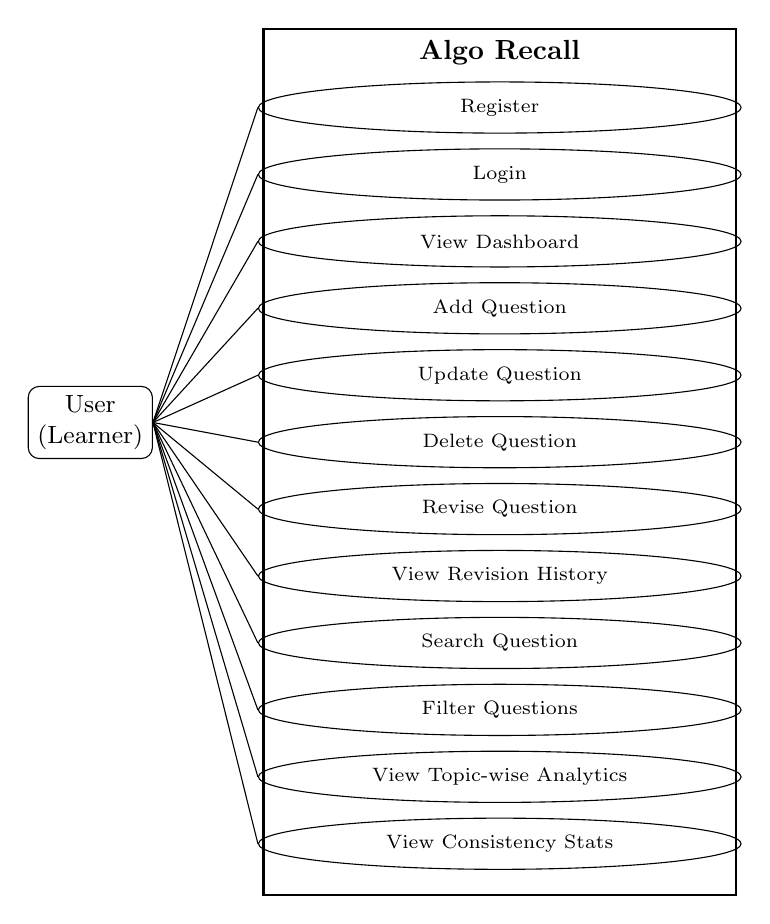
\begin{tikzpicture}[
    actorbox/.style={
        draw,
        rounded corners,
        minimum width=1.5cm,
        minimum height=0.8cm,
        align=center,
        font=\small
    },
    usecase/.style={
        draw,
        ellipse,
        minimum width=4.4cm,
        minimum height=0.65cm,
        text width=4.1cm,
        align=center,
        font=\scriptsize
    }
]

% Actor
\node[actorbox] (actor) at (0,0) {User\\(Learner)};

% System boundary
\draw[thick] (2.2,-6.0) rectangle (8.2,5.0);
\node[font=\bfseries] at (5.2,4.7) {Algo Recall};

% Use cases: uniform size and spacing
\node[usecase] (uc1)  at (5.2,4.0) {Register};
\node[usecase] (uc2)  at (5.2,3.15) {Login};
\node[usecase] (uc3)  at (5.2,2.3) {View Dashboard};
\node[usecase] (uc4)  at (5.2,1.45) {Add Question};
\node[usecase] (uc5)  at (5.2,0.6) {Update Question};
\node[usecase] (uc6)  at (5.2,-0.25) {Delete Question};
\node[usecase] (uc7)  at (5.2,-1.1) {Revise Question};
\node[usecase] (uc8)  at (5.2,-1.95) {View Revision History};
\node[usecase] (uc9)  at (5.2,-2.8) {Search Question};
\node[usecase] (uc10) at (5.2,-3.65) {Filter Questions};
\node[usecase] (uc11) at (5.2,-4.5) {View Topic-wise Analytics};
\node[usecase] (uc12) at (5.2,-5.35) {View Consistency Stats};

% Association lines
\foreach \n in {uc1,uc2,uc3,uc4,uc5,uc6,
                uc7,uc8,uc9,uc10,uc11,uc12}
{
    \draw[thin] (actor.east) -- (\n.west);
}

\end{tikzpicture}
\caption{Algo Recall V1 use-case diagram}
\label{fig:usecase}
\end{figure}


\textbf{Use cases and descriptions}

\begin{longtable}{|>{\centering\arraybackslash}p{0.08\textwidth}|p{0.25\textwidth}|p{0.57\textwidth}|}
\hline
\textbf{No.} & \textbf{Use Case} & \textbf{Description}\\ \hline
1 & Register & Creates a new account on Algo Recall.\\ \hline
2 & Login & Authenticates the user and grants access to their account.\\ \hline
3 & View Dashboard & Displays the day's suggested revision questions and revision completion progress.\\ \hline
4 & Add Question & Stores a solved DSA question with its details, confidence level, and revision information.\\ \hline
5 & Update Question & Modifies the stored details of an existing question.\\ \hline
6 & Delete Question & Removes a question from the user's stored collection.\\ \hline
7 & Revise Question & Marks a suggested question as revised and updates its confidence level and revision details.\\ \hline
8 & View Revision History & Displays previous revision sessions and their recorded details.\\ \hline
9 & Search Question & Finds a stored question using its name or other searchable information.\\ \hline
10 & Filter Questions & Filters stored questions by topic, difficulty, or other supported attributes.\\ \hline
11 & View Topic-wise Analytics & Displays revision and confidence statistics for different DSA topics.\\ \hline
12 & View Consistency Stats & Shows revision activity over time so the user can track consistency.\\ \hline
\end{longtable}

\subsection{Use Case Templates}
\textbf{Use Case ID: UC-07}\\
\textbf{Name:} Revise Question\\
\textbf{Primary actor:} User (Learner)

\textbf{Preconditions}
\begin{itemize}
\item The learner is logged in.
\item The question exists in the learner's collection.
\end{itemize}

\textbf{Trigger:} The learner chooses a suggested question to revise.

\textbf{Main flow}
\begin{enumerate}
\item The learner opens the dashboard and selects a suggested question.
\item The learner revises the question.
\item The learner submits a confidence rating.
\item The system updates the question's confidence and revision details.
\item The system records the revision in history and updates the next-revision schedule.
\end{enumerate}

\textbf{Alternative flow:} If the confidence rating is invalid or the question cannot be
found, the system returns an error instead of recording the revision.

\textbf{Postconditions:} The question and revision history reflect the recorded revision.
The exact scheduling formula is not specified in the V1 reference.

\section{Activity Diagram and Swimlane Diagrams}
This activity diagram illustrates the high-level revision workflow. It can be expanded
into swimlanes for the learner, application, and database if required.

\begin{figure}[htbp]
\centering
\begin{tikzpicture}[
node distance=0.55cm,
startstop/.style={draw,rounded rectangle,minimum width=3cm,minimum height=0.6cm,align=center},
process/.style={draw,rectangle,minimum width=4.2cm,minimum height=0.65cm,align=center},
decision/.style={draw,diamond,aspect=2.1,inner sep=1pt,align=center},
flow/.style={-Latex}
]
\node[startstop] (start) {Start};
\node[process,below=of start] (dashboard) {Open dashboard};
\node[process,below=of dashboard] (choose) {Select suggested question};
\node[process,below=of choose] (revise) {Revise question and enter confidence};
\node[decision,below=0.8cm of revise] (valid) {Rating valid?};
\node[process,below left=0.9cm and 0.3cm of valid] (invalid) {Show validation error};
\node[process,below right=0.9cm and 0.3cm of valid] (save) {Update question and history};
\node[startstop,below=0.8cm of save] (finish) {Update schedule and progress};
\draw[flow] (start) -- (dashboard);
\draw[flow] (dashboard) -- (choose);
\draw[flow] (choose) -- (revise);
\draw[flow] (revise) -- (valid);
\draw[flow] (valid) -- node[above left]{No} (invalid);
\draw[flow] (valid) -- node[above right]{Yes} (save);
\draw[flow] (invalid.west) -| ([xshift=-1.8cm]choose.west) |- (choose.west);
\draw[flow] (save) -- (finish);
\end{tikzpicture}
\caption{Activity diagram for revising a question}
\label{fig:activity}
\end{figure}

\section{Data Flow Diagrams (DFDs)}
These diagrams are illustrative and show broad data interactions. They should be checked
against the final implementation before submission.

\subsection{DFD Level 0}

\begin{figure}[htbp]
\centering
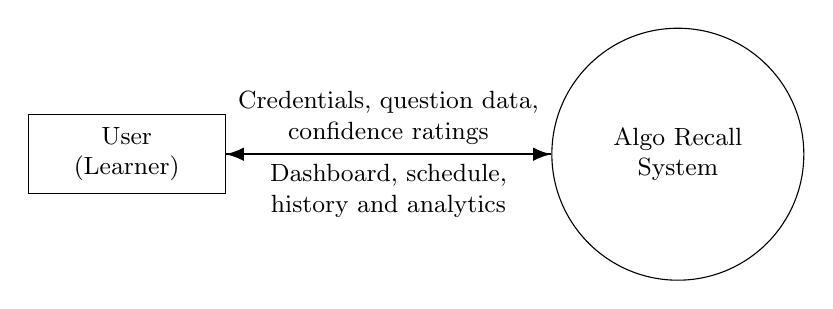
\begin{tikzpicture}[
    entity/.style={
        draw,
        rectangle,
        minimum width=2.5cm,
        minimum height=1cm,
        align=center,
        font=\small
    },
    process/.style={
        draw,
        circle,
        minimum size=3.2cm,
        align=center,
        font=\small
    },
    flow/.style={-{Latex}, thick}
]

% User and system
\node[entity] (learner) at (0,0) {User\\(Learner)};
\node[process] (system) at (7,0) {Algo Recall\\System};

% Input flow
\draw[flow]
    (learner.east) --
    node[above, align=center, text width=4cm, font=\small]
    {Credentials, question data,\\confidence ratings}
    (system.west);

% Output flow
\draw[flow]
    (system.west) --
    node[below, align=center, text width=4cm, font=\small]
    {Dashboard, schedule,\\history and analytics}
    (learner.east);

\end{tikzpicture}
\caption{DFD Level 0: Algo Recall context diagram}
\label{fig:dfd0}
\end{figure}


\subsection{DFD Level 1}

\begin{figure}[htbp]
\centering
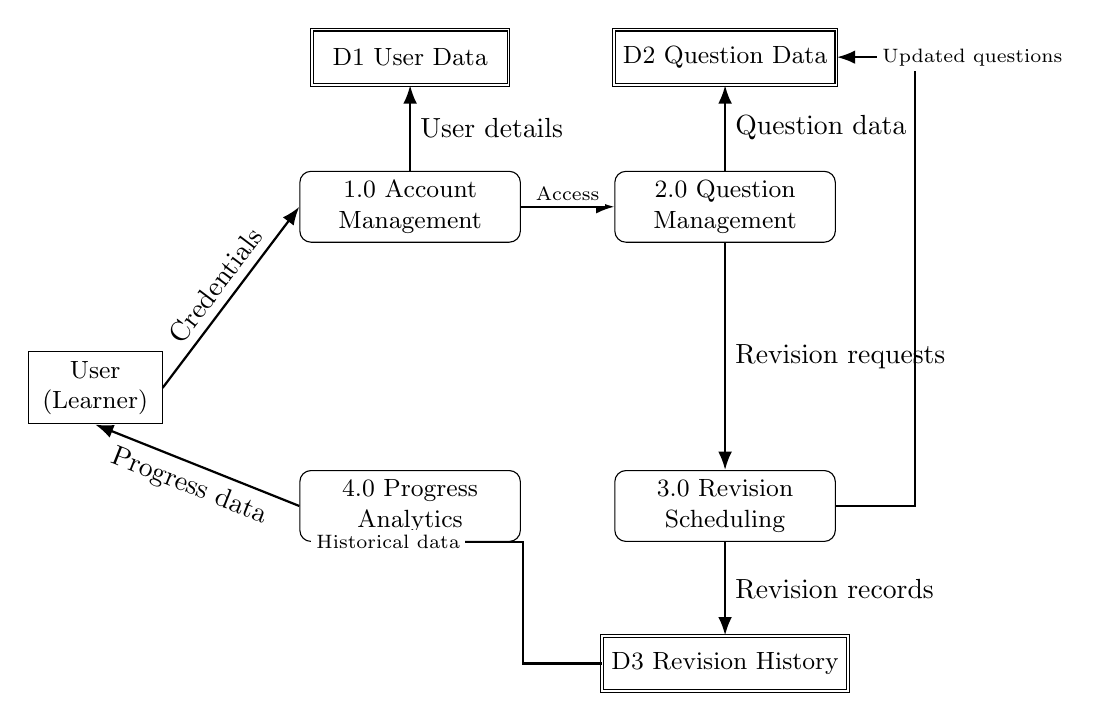
\begin{tikzpicture}[
    process/.style={
        draw, rounded corners,
        minimum width=2.8cm,
        minimum height=0.9cm,
        align=center, font=\small
    },
    store/.style={
        draw, double,
        minimum width=2.5cm,
        minimum height=0.7cm,
        align=center, font=\small
    },
    entity/.style={
        draw, rectangle,
        minimum width=1.7cm,
        minimum height=0.8cm,
        align=center, font=\small
    },
    flow/.style={-{Latex}, thick},
    every edge quotes/.style={
        font=\scriptsize,
        fill=white,
        inner sep=2pt,
        align=center
    }
]

% User
\node[entity] (user) at (0,1.5)
    {User\\(Learner)};

% Processes
\node[process] (auth) at (4,3.8)
    {1.0 Account\\Management};

\node[process] (manage) at (8,3.8)
    {2.0 Question\\Management};

\node[process] (analytics) at (4,0)
    {4.0 Progress\\Analytics};

\node[process] (schedule) at (8,0)
    {3.0 Revision\\Scheduling};

% Data stores
\node[store] (users) at (4,5.7)
    {D1 User Data};

\node[store] (questions) at (8,5.7)
    {D2 Question Data};

\node[store] (history) at (8,-2)
    {D3 Revision History};

% User interactions
\draw[flow] (user.east) --
    node[above, sloped, pos=0.5]
    {Credentials} (auth.west);

\draw[flow] (analytics.west) --
    node[below, sloped, pos=0.5]
    {Progress data} (user.south);

% Account management
\draw[flow] (auth.north) --
    node[right] {User details} (users.south);

\draw[flow] (auth.east) --
    node[above, font=\scriptsize, fill=white, inner sep=2pt]
    {Access}
    (manage.west);

% Question management
\draw[flow] (manage.north) --
    node[right] {Question data}
    (questions.south);

% Revision scheduling
\draw[flow] (manage.south) --
    node[right] {Revision requests}
    (schedule.north);

\draw[flow] (schedule.east) -- ++(1,0)
    |- (questions.east)
    node[pos=0.75, right, font=\scriptsize,
         fill=white, inner sep=2pt]
    {Updated questions};

% Revision history
\draw[flow] (schedule.south) --
    node[right] {Revision records}
    (history.north);

\draw[flow] (history.west) --
    ++(-1,0) |- 
    node[pos=0.75, left, font=\scriptsize,
         fill=white, inner sep=2pt]
    {Historical data}
    (analytics.south);

\end{tikzpicture}

\caption{DFD Level 1: Main processes and data stores}
\label{fig:dfd1}
\end{figure}


\subsection{DFD Level 2}
This example expands the revision-scheduling process:
\begin{enumerate}
\item Receive the selected question and confidence rating.
\item Validate the rating and verify question ownership.
\item Calculate the next revision date and priority.
\item Save the updated question and create a revision-history record.
\item Return the updated question and confirmation to the learner.
\end{enumerate}

The V1 reference states that the dashboard should suggest approximately 5--7 questions per
day. Unfinished suggested questions should carry forward alongside newly scheduled
questions, and the visible workload should not grow without control. The exact mechanism
for controlling this workload is not specified and should be documented once decided.

\section{Software Requirement Specification in IEEE Format}
This concise draft is based on the supplied V1 scope. Expand it if the course requires a
specific IEEE SRS template.

\subsection*{1. Introduction}
\textbf{Purpose:} Specify the user-facing requirements for Algo Recall V1.

\textbf{Scope:} Algo Recall allows learners to manage solved DSA questions, revise them using
confidence-based scheduling, and monitor revision progress and consistency.

\subsection*{2. Overall Description}
\textbf{Primary user:} User (Learner).

\textbf{Included functions:} Registration, login, dashboard, question management, revision,
revision history, search, filtering, topic-wise analytics, and consistency statistics.

\textbf{Excluded from V1:} Online judge or code execution, contest management, AI-generated
solutions, and automatic LeetCode synchronisation.

\subsection*{3. Functional Requirements}
\begin{itemize}
\item FR-1: The system shall allow a learner to register for an account.
\item FR-2: The system shall allow a learner to log in.
\item FR-3: The system shall display suggested revision questions and completion progress.
\item FR-4: The system shall allow a learner to add, update, and delete stored questions.
\item FR-5: The system shall allow a learner to record a revision and confidence rating.
\item FR-6: The system shall provide revision history.
\item FR-7: The system shall support question search and filtering by supported attributes.
\item FR-8: The system shall display topic-wise revision and confidence statistics.
\item FR-9: The system shall display revision activity over time.
\item FR-10: The dashboard should target approximately 5--7 suggested questions per day,
carry unfinished questions forward, and prevent the visible workload from growing without control.
\end{itemize}

\subsection*{4. Non-Functional Requirements}

\begin{itemize}
    \item Usability: The system should provide a simple and user-friendly interface for managing DSA questions and revision activities.
\end{itemize}
\begin{itemize}
    \item Security: Users should only be able to access and modify their own data.
\end{itemize}
\begin{itemize}
    \item Reliability: The system should store question details and revision history accurately.
\end{itemize}
\begin{itemize}
    \item Performance: The system should handle routine operations such as adding, updating, searching, and revising questions efficiently.
\end{itemize}
 \begin{itemize}
     \item Maintainability: The system should have a modular code structure that allows future updates and modifications easily.
 \end{itemize}

\section{User Stories and Story Cards}
The following sample stories are based on the listed V1 use cases.

\begin{longtable}{|>{\centering\arraybackslash}p{0.12\textwidth}|p{0.70\textwidth}|p{0.12\textwidth}|}
\hline
\textbf{ID} & \textbf{User Story} & \textbf{Priority}\\ \hline
US-01 & As a learner, I want to register and log in so that I can access my account. & High\\ \hline
US-02 & As a learner, I want to add, update, and delete DSA questions so that I can manage my solved-question collection. & High\\ \hline
US-03 & As a learner, I want to record my confidence after revising a question so that its revision details can be updated. & High\\ \hline
US-04 & As a learner, I want to see today's suggested questions and completion progress so that I can plan my revision. & High\\ \hline
US-05 & As a learner, I want to search and filter questions so that I can find a question quickly. & Medium\\ \hline
US-06 & As a learner, I want to view revision history so that I can review previous sessions. & Medium\\ \hline
US-07 & As a learner, I want topic-wise analytics and consistency statistics so that I can monitor progress. & Medium\\ \hline
\end{longtable}

\textbf{Example story card — US-03: Record confidence after revision}

\textbf{Acceptance criteria}
\begin{itemize}
\item The learner can submit a confidence rating.
\item The system validates the rating according to the application's supported range.
\item A valid rating updates the question's confidence and revision details.
\item The system records the revision in revision history.
\end{itemize}

% -------------------- REFERENCES --------------------
\begin{thebibliography}{9}
\bibitem{node} OpenJS Foundation, \textit{Node.js Documentation}. Available at:
\url{https://nodejs.org/docs/}
\bibitem{express} Express.js, \textit{Express Documentation}. Available at:
\url{https://expressjs.com/}
\bibitem{mongodb} MongoDB, \textit{MongoDB Manual}. Available at:
\url{https://www.mongodb.com/docs/}
\end{thebibliography}

\end{document}
